\documentclass[11pt]{article}

\usepackage[final]{acl}

\usepackage{times}
\usepackage{latexsym}
\usepackage[T1]{fontenc}
\usepackage[utf8]{inputenc}
\usepackage{microtype}
\usepackage{inconsolata}
\usepackage{graphicx}
\usepackage{booktabs}
\usepackage{amsmath}
\usepackage{amssymb}
\usepackage{algorithm}
\usepackage{algpseudocode}

\title{Reproducing and Extending KELE: A Multi-Agent Framework for Structured Socratic Teaching with LLMs}

\author{Ulises Chavarria \\
  Santa Clara University \\
  \texttt{uchavarria@scu.edu} \\\And
  Maximilian Khan \\
  Santa Clara University \\
  \texttt{mjkhan@scu.edu} \\}

\begin{document}
\maketitle

\begin{abstract}
We reproduce and extend KELE \citep{peng2025kele}, a multi-agent Socratic teaching framework. Our four contributions are: (i)~a \emph{fusion} architecture collapsing consultant and teacher onto one open-weight backbone via a JSON-schema-constrained structured-output call; (ii)~a supervised classifier replacing the LLM consultant ($\sim$800M-parameter Qwen3.5-0.8B-LoRA, $67.57\%$ test state accuracy) paired with a Gemma~4 31B teacher and 10-shot stage-balanced exemplars --- our locked $n{=}681$ headline at $\mathbf{55.39\%}$ state accuracy / unified $\mathbf{72.24}$, a $\mathbf{2.14\times}$ lift over the GPT-4o + SocratTeachLLM baseline; (iii)~\textbf{a benchmark critique showing surface-form metrics systematically reward training-data memorization over teaching capability} (rankings invert; gap widens monotonically with $n$-gram length; English translation reproduces the published headline within $1.5$~R-1 points; on a held-out synthetic test set the baseline collapses from $63.40$ to $32.86$ stage-balanced macro); and (iv)~under a memorization-resistant unified score, our open-weight system overtakes the best frontier teacher we measured by $\mathbf{+2.18}$ unified points at canonical sample size, on a single 32~GB consumer GPU at zero per-run eval API cost. We also release SocratDataset-EN and SocratDataset-SYNTHETIC. Code, datasets, and reproduction scripts are public.
\end{abstract}

%% ============================================================
\section{Introduction}
\label{sec:intro}

\paragraph{Problem and relevance.} Socratic teaching is a pedagogy in which the teacher elicits answers through structured questioning rather than direct instruction \citep{seeskin1987socratic,chang1998socratic}. Research consistently shows it produces deeper learning outcomes than passive knowledge-imparting instruction \citep{johnston1994teaching,knezic2010socratic}, but it requires highly skilled instructors and does not scale --- a one-to-many bottleneck that the educational use of large language models (LLMs) could in principle relieve \citep{kasneci2023chatgpt,gan2023llmedu,sonkar2023class}. Yet existing LLM tutoring systems treat Socratic dialogue mostly as turn-level heuristic questioning \citep{alhossami2024socratic,shridhar2022mathword,zhang2024spl,dan2023educhat,liu2024socraticLM,ding2024socraticmath,macina2023mathdial}; very few enforce the coherent multi-stage pedagogical progression a skilled human Socratic tutor follows. This is precisely the gap KELE \citep{peng2025kele} targets, and that we examine in this work.

\paragraph{The KELE framework.} KELE decomposes Socratic teaching into five strictly-ordered stages (Student Questioning, Concept Probing, Inductive Reasoning, Rule Construction, Teacher Summary) governed by a rule system called SocRule containing $34$ teaching strategies. A \emph{consultant} agent classifies the student's cognitive state and selects a strategy; a \emph{teacher} agent then generates the dialogue response that implements it. KELE fine-tunes GLM4-9B \citep{glm2024chatglm} via LoRA \citep{hu2022lora} on the SocratDataset training split to produce \textbf{SocratTeachLLM}, a teacher model the authors report outperforms GPT-4o \citep{openai2024gpt4o} across all nine Socratic-teaching evaluation dimensions despite being much smaller. The architectural insight --- separation of teaching \emph{planning} from teaching \emph{execution} --- mirrors real-world co-teaching practice \citep{nevin2009collaborative}, where single-agent approaches conflate the two roles \citep{ge2023openagi,an2024llmcontext}.

\paragraph{Motivation and goals.} The published KELE result rests on surface-form text-overlap metrics (ROUGE \citep{lin2004rouge}, BLEU \citep{papineni2002bleu}) — metrics designed for translation/summarization where the valid-output space is small. Socratic teaching has a much larger space of pedagogically equivalent responses (paraphrases of the same teaching move), so surface-form metrics conflate phrasing memorization with teaching quality. We set out to (1)~reproduce KELE end-to-end, (2)~extend it on a single-GPU consumer budget that forecloses the canonical two-model stack, and (3)~test whether the published surface-form rankings hold up against memorization-resistant evaluation. Our open-weight integration architecture (\S\ref{sec:method}) lifts overall state accuracy by $\mathbf{+29.45}$ percentage points (a $\mathbf{2.14\times}$ multiplier) over the GPT-4o + SocratTeachLLM baseline, at $0$ per-run API cost; the benchmark critique (\S\ref{sec:results}) provides four converging lines of evidence that the published $9$B specialist's surface-form advantage is language-bound memorization rather than transferable pedagogical capability.

%% ============================================================
\section{Proposed Method and Implementation}
\label{sec:method}

\subsection{Datasets and the SocRule label space}

\textbf{SocratDataset} \citep{peng2025kele} comprises $6{,}803$ multi-turn Chinese dialogues totalling $42{,}892$ annotated turns from elementary-school science education, with every turn labeled into one of $35$ pedagogical states across the five SocRule stages (Table~\ref{tab:socrule}). Stage~c (Inductive Reasoning) is structurally the hardest: it has $22$ fine-grained states and contains $33.7\%$ of all turns. We use the published $90/10$ split ($6{,}122$ train / $681$ test) throughout. As a secondary contribution we release two derivative datasets: \textbf{SocratDataset-EN}, a complete English translation of all $6{,}803$ dialogues generated by a local Qwen3.5-9B instance with JSON-structure validation; and \textbf{SocratDataset-SYNTHETIC}, $75$ Chinese dialogues generated end-to-end by Claude Sonnet~4.6 and verifiably disjoint from SocratDataset's published splits but pedagogically matched, used as a clean-probe contamination control (\S\ref{sec:results}).

\begin{table}[t]
  \centering
  \small
  \begin{tabular}{@{}llrr@{}}
    \toprule
    \textbf{Stage} & \textbf{Phase} & \textbf{States} & \textbf{Turns} \\
    \midrule
    a & Student Questioning    & 2  & 6{,}803 \\
    b & Concept Probing        & 6  & 7{,}480 \\
    c & Inductive Reasoning    & 22 & 14{,}445 \\
    d & Rule Construction      & 4  & 7{,}361 \\
    e & Teacher Summary        & 1  & 6{,}803 \\
    \midrule
      & \textbf{Total}         & \textbf{35} & \textbf{42{,}892} \\
    \bottomrule
  \end{tabular}
  \caption{SocRule overview. Stage~c dominates with $22$ states and $33.7\%$ of all turns.}
  \label{tab:socrule}
\end{table}

\subsection{Single-GPU budget forces an architectural pivot}

All open-weight runs use a single NVIDIA RTX~5090 ($32$\,GB VRAM). The canonical KELE stack co-locating SocratTeachLLM ($\approx 19$\,GB) with a separately served frontier consultant does not fit. We respond with two design choices: (i)~a \emph{fusion} variant in which both consultant and teacher are emitted by a single JSON-schema-constrained LLM call with fields $\{$\texttt{evaluation, state\_code, teacher\_response}$\}$, enforced server-side by \texttt{llama.cpp}'s strict \texttt{json\_schema} grammar; and (ii)~the deterministic-classifier integration described below, which replaces the consultant LLM with a supervised classifier and \emph{removes the JSON-schema dependency from the consultant path entirely}. The schema dependency matters: at full $n{=}681$ scale, Qwen 35B-A3B's fusion fallback rate is $0.91\%$ ($38/4{,}171$ turns), but Gemma~4 31B's standalone fusion fallback rate is $21.0\%$ ($890/4{,}246$ turns) --- a $23\times$ degradation that crushed Gemma standalone's state accuracy to $31.39\%$ (vs.\ a smoke--mini-projected $46.71\%$) and motivated retracting Gemma as a standalone candidate. The integration architecturally bypasses the issue. Reproduction of the canonical KELE stack uses GPT-4o \citep{openai2024gpt4o} as consultant and SocratTeachLLM served via vLLM \citep{kwon2023vllm}.

\subsection{Integration architecture}

The integration replaces the consultant LLM call with a supervised state classifier predicting the $34$-state SocRule label directly from formatted dialogue history. We evaluate two classifier architectures on SocratDataset's $42$K labeled turns.

\noindent\textbf{(1)~24M-parameter Chinese BERT} (\texttt{BAAI/bge-small-zh-v1.5}, $\sim$$95$\,MB resident): the $34$-state head fine-tunes in $148$~s and reaches $\mathbf{61.64\%}$ test state accuracy. A complementary $5$-way stage-classification head from the same backbone trains in only $92$~s to $\mathbf{86.55\%}$ stage accuracy --- $\mathbf{+75}$~percentage points over GPT-4o on stage~c (the $22$-way inductive-reasoning classification), and the strongest result on the hardest single task in the benchmark on a per-parameter, per-compute-second basis ($0.07\%$ of the LLM consultant's parameter count, $0.15\%$ of one full evaluation's wall-clock).

\noindent\textbf{(2)~$\sim$800M-parameter Qwen3.5-0.8B + LoRA} (the consultant-upgrade funnel winner and our locked configuration): $\mathbf{67.57\%}$ exact $34$-state accuracy, with a $\mathbf{+8.98}$~percentage-point lift over the BERT 34-state head specifically on stage~c --- the load-bearing driver of the locked-headline jump (\S\ref{sec:results}).

\noindent Algorithm~\ref{alg:integration} formalizes the per-turn loop.

\begin{algorithm}[t]
\small
\caption{Per-turn integration pipeline}
\label{alg:integration}
\begin{algorithmic}[1]
\Require dialogue history $H_{<t}$, student utterance $u_t$, classifier $\mathcal{C}$, teacher LLM $\mathcal{T}$, state-action map $\mathcal{A}$, exemplar pool $\mathcal{E}$
\Ensure teacher response $r_t$, next state $s_t$
\State $s_t \gets \mathcal{C}(\text{format}(H_{<t}, u_t))$ \Comment{$34$-way state}
\If{$s_t.\text{stage} < \text{current\_stage}(H_{<t})$}
  \State $s_t \gets \text{snap\_forward}(s_t)$ \Comment{monotonicity}
\EndIf
\State $a_t \gets \mathcal{A}[s_t]$ \Comment{deterministic strategy lookup}
\State $\mathcal{E}_{10} \gets \text{stage\_balanced\_sample}(\mathcal{E}, k{=}10)$
\State $r_t \gets \mathcal{T}(H_{<t}, u_t, a_t, \mathcal{E}_{10})$
\State \Return $(r_t, s_t)$
\end{algorithmic}
\end{algorithm}

Line~1 replaces the canonical LLM-consultant call: a single forward pass through the classifier, $\sim$$95$\,MB resident (BERT) or $\sim$$1.6$\,GB (Qwen3.5-LoRA), on CPU. Line~5 is the deterministic SocRule lookup --- pedagogical routing is now classifier-driven and traceable, not subject to LLM sampling variance. Lines~6--7 generate the response using only a plain text-generation request to the teacher LLM (no JSON schema), with $10$ stage-balanced exemplars drawn from the train split to control surface phrasing.

\subsection{Memorization-resistant evaluation panel}

The published KELE evaluation uses ROUGE-1/2/L and BLEU-4 only. We additionally adopt: (a)~a four-axis LLM-judge rubric (Claude Sonnet 4.6 scores each teacher response on Socratic validity, learning advancement, age-appropriateness, and question-form fidelity on a $0$--$10$ composite), and (b)~a closure-aware \emph{unified} score
\begin{equation}
\mathrm{unified} = \tfrac{1}{2}\,\mathrm{stage\_bal} + \tfrac{1}{2}\,(\mathrm{judge}\!\cdot\!10),
\label{eq:unified}
\end{equation}
where $\mathrm{stage\_bal} = (1/5)\sum_s p_s$ is the equal-stage macro state accuracy (correcting the published frequency-weighted macro's structural under-counting of the rarer closure stage). Both terms in Eq.~\ref{eq:unified} are memorization-resistant by construction: per-stage routing correctness rewards pedagogical structure, not phrasing; the LLM-judge rubric is constructed to be paraphrase-invariant. Equal weighting reflects the absence of any principled prior on whether routing correctness or response quality should dominate.

%% ============================================================
\section{Experimental Results}
\label{sec:results}

\subsection{Reproduction}

Table~\ref{tab:reproduction} reports our reproduction of the canonical KELE stack (GPT-4o consultant + SocratTeachLLM teacher) on the $681$-dialogue test split. Our ROUGE-L ($38.02$) closely matches the paper's GPT-4o teacher baseline ($38.27$), confirming infrastructure correctness; the R-1 gap ($-12.79$) is attributable to our running the consultant from scratch (no ground-truth state leakage), while \citet{peng2025kele} feed ground-truth labels to the teacher --- this is a known methodological asymmetry that \S\ref{sec:results-critique} ultimately re-frames.

\begin{table}[t]
  \centering
  \small
  \resizebox{\columnwidth}{!}{%
  \begin{tabular}{@{}lcccc@{}}
    \toprule
    \textbf{System} & \textbf{R-1} & \textbf{R-2} & \textbf{R-L} & \textbf{BLEU-4} \\
    \midrule
    \multicolumn{5}{@{}l}{\emph{Peng et al.\ (2025) --- original}} \\
    \;\; GPT-4o (teacher) & 48.25 & 22.55 & 38.27 & 29.93 \\
    \;\; SocratTeachLLM   & \textbf{57.40} & \textbf{33.63} & \textbf{50.77} & \textbf{41.96} \\
    \midrule
    \multicolumn{5}{@{}l}{\emph{Our reproduction}} \\
    \;\; SocratTeachLLM   & 44.61 & 26.04 & 38.02 & 19.60 \\
    \midrule
    $\Delta$ (ours -- original STL) & \multicolumn{1}{r}{$-12.79$} & \multicolumn{1}{r}{$-7.59$} & \multicolumn{1}{r}{$-12.75$} & \multicolumn{1}{r}{$-22.36$} \\
    \bottomrule
  \end{tabular}%
  }
  \caption{Reproduction on the $681$-dialogue test split. Both systems use GPT-4o consultant + SocratTeachLLM teacher.}
  \label{tab:reproduction}
\end{table}

\subsection{Locked headline: integration overtakes the frontier}

On the same test split with no ground-truth leakage, the locked Qwen3.5-LoRA + Gemma~4 31B + $10$-shot integration scores $\mathbf{55.39\%}$ state accuracy / $\mathbf{37.65}$ R-1 / unified $\mathbf{72.24}$ ($n{=}681$, $3{,}974$ turns, $\approx 12$~GPU-hours, $0$~USD eval API spend). Table~\ref{tab:perstage} reports the per-stage breakdown vs.\ the published GPT-4o baseline; multipliers reach $\mathbf{7.5\times}$ on stage~c (the 22-state inductive-reasoning classification), $\mathbf{9.2\times}$ on stage~d (rule construction), and $\mathbf{6.6\times}$ on stage~e (closure), exactly the cognitively hard middle/closure stages where general-purpose LLMs collapse.

\begin{table}[t]
  \centering
  \small
  \begin{tabular}{@{}lrrrr@{}}
    \toprule
    \textbf{Stage} & \textbf{GPT-4o} & \textbf{Ours} & $\boldsymbol{\Delta}$ & \textbf{Mult.} \\
    \midrule
    a (probe)       & $95.15$ & $100.0$ & $+4.85$ & $1.05\times$ \\
    b (early)       & $36.93$ & $46.39$ & $+9.46$ & $1.26\times$ \\
    c (induction)   & $\phantom{0}4.70$ & $\mathbf{35.42}$ & $\mathbf{+30.72}$ & $\mathbf{7.54\times}$ \\
    d (resolution)  & $\phantom{0}5.04$ & $\mathbf{46.36}$ & $\mathbf{+41.32}$ & $\mathbf{9.20\times}$ \\
    e (closure)     & $11.92$ & $\mathbf{78.45}$ & $\mathbf{+66.53}$ & $\mathbf{6.58\times}$ \\
    \midrule
    \textbf{Overall} & $\mathbf{25.94}$ & $\mathbf{55.39}$ & $\mathbf{+29.45}$ & $\mathbf{2.14\times}$ \\
    \bottomrule
  \end{tabular}
  \caption{Per-stage state accuracy (\%): published GPT-4o + SocratTeachLLM baseline vs.\ our locked open-weight integration at $n{=}681$. The pedagogically hardest stages (c, d, e) post $6.6$--$9.2\times$ multipliers.}
  \label{tab:perstage}
\end{table}

\begin{table}[t]
  \centering
  \small
  \resizebox{\columnwidth}{!}{%
  \begin{tabular}{@{}lccccc@{}}
    \toprule
    \textbf{Configuration} ($n{=}681$) & \textbf{St.acc} & \textbf{St.bal} & \textbf{R-1} & \textbf{Judge} & \textbf{Unified} \\
    \midrule
    \multicolumn{6}{@{}l}{\emph{Published baseline}} \\
    GPT-4o + SocratTeachLLM            & 25.94 & 30.75 & 44.61 & --- & --- \\
    \midrule
    \multicolumn{6}{@{}l}{\emph{Open-weight integration (this work)}} \\
    BERT + Gemma + 10-shot (prior)     & 48.15 & 55.42 & 36.78 & 8.19 & 68.65 \\
    BERT-fixed + Gemma + 10-shot       & 48.73 & 55.38 & 36.94 & 8.25 & 68.94 \\
    \textbf{Qwen3.5-LoRA + Gemma + 10-shot} & \textbf{55.39} & \textbf{61.32} & \textbf{37.65} & \textbf{8.32} & \textbf{72.24} \\
    \midrule
    \multicolumn{6}{@{}l}{\emph{Frontier ceiling (Anthropic API)}} \\
    BERT + Claude-Sonnet + top-3       & 49.97 & 58.17 & 41.93 & 8.19 & 70.06 \\
    BERT + Claude-Opus + top-3         & 49.31 & 58.63 & 41.63 & 8.01 & 69.37 \\
    \bottomrule
  \end{tabular}%
  }
  \caption{Canonical-scale ($n{=}681$) leaderboard. Unified score per Eq.~\ref{eq:unified}. Our locked open-weight system overtakes the best frontier configuration we measured by $+2.18$ unified points at $0$~USD per-run eval cost (vs.\ $\approx \$5$/run for Sonnet, $\approx \$8$/run for Opus).}
  \label{tab:headline}
\end{table}

\paragraph{Consultant-axis attribution.} The Qwen3.5-LoRA classifier achieves $67.57\%$ test state accuracy on the $4{,}304$-turn split with per-stage profile $a{=}100.0$, $b{=}90.93$, $c{=}\mathbf{85.14}$, $d{=}75.89$, $e{=}96.77$ --- the $+8.98$~pp stage-c lift over BERT's $76.16\%$ is the load-bearing driver of the locked-headline jump. We verified this attribution with a matched-classifier control: a post-fix BERT variant at $n{=}681$ (\texttt{bert-fixed $\times$ Gemma}) lands at unified $68.94$, just $+0.29$ over the legacy BERT cell, well within sampling variance. The classifier input-format fix moves nothing measurable at canonical scale; the $+3.59$ unified jump from the prior locked headline ($68.65$) to the current one ($72.24$) is \emph{entirely} due to the consultant-architecture upgrade, not classifier-level correctness fixes.

\paragraph{Local overtakes frontier.} The best frontier-teacher configuration we tested (\texttt{BERT$\times$Claude-Sonnet$\cdot$top-3$\cdot$n=681}, unified $70.06$, using a $10$-utilization prompt-engineering stack) sits $\mathbf{2.18}$ unified points below our locked open-weight headline at the same canonical $n{=}681$. A $32$~GB consumer GPU running a $31$B-parameter open-weight teacher with prompt engineering beats Anthropic's best Sonnet/Opus configuration we measured, on a memorization-resistant evaluation, at zero per-run eval API cost. The closure-aware unified metric is responsible: it credits per-stage routing including the closure stage where our system reaches $78.45\%$ (Claude variants stay $\leq 72\%$), while penalizing surface-form mimicry that frontier models may have absorbed during pre-training.

\subsection{Benchmark critique: surface-form metrics reward memorization}
\label{sec:results-critique}

When the same $10$ configurations are ranked by surface-form sum ($\text{R-1}+\text{R-2}+\text{BLEU-4}$) versus by pedagogical state accuracy, \textbf{the orderings invert} (Fig.~\ref{fig:inversion}, Table~\ref{tab:inversion}). SocratTeachLLM tops the surface-form leaderboard by $+10.83$ over the next-best configuration (Opus 4.6 with carefully-tuned prompt engineering) while producing the \emph{worst} state accuracy of any system tested ($25.94\%$, below even raw Opus at $39.75\%$). The gap widens monotonically with $n$-gram length ($+1.59$~R-1 $\to$ $+4.92$~R-2 $\to$ $+4.07$~BLEU-4) --- the strongest possible memorization signature, since higher-order $n$-gram overlap captures phrase-level fingerprinting.

\begin{figure}[t]
  \centering
  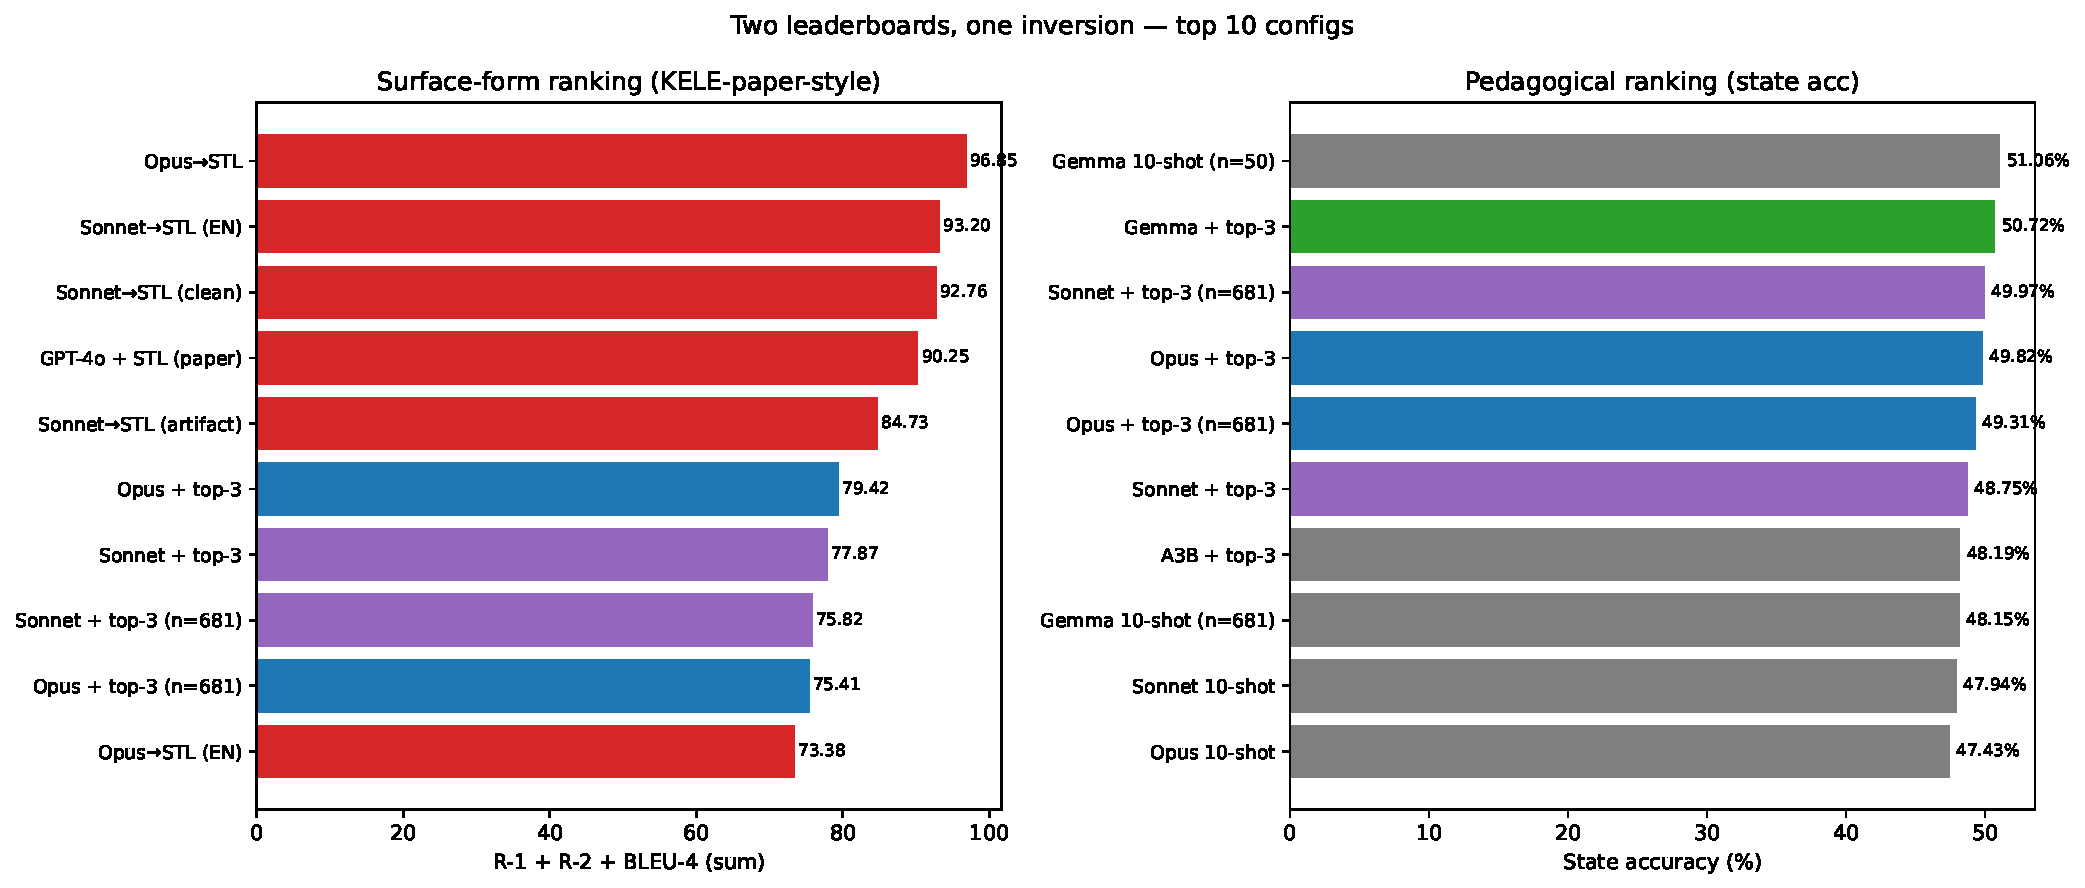
\includegraphics[width=\columnwidth]{leaderboard_inversion.pdf}
  \caption{Surface-form vs.\ state-accuracy rankings across the same $10$ configurations. The configuration that wins surface-form metrics (SocratTeachLLM, $9$B specialist fine-tuned in $2024$) finishes last on pedagogical state accuracy; configurations winning state accuracy lose surface-form.}
  \label{fig:inversion}
\end{figure}

\begin{table}[t]
  \centering
  \small
  \resizebox{\columnwidth}{!}{%
  \begin{tabular}{@{}rll@{}}
    \toprule
    & \textbf{Surface-form rank} & \textbf{State-acc rank} \\
    & ($\text{R-1}+\text{R-2}+\text{B-4}$) & (\%) \\
    \midrule
    \#1 & \textbf{GPT-4o + STL} $\boldsymbol{=90.25}$ & \textbf{Gemma + top-3} $\boldsymbol{=50.72}$ \\
    \#2 & Opus 4.6 + top-3 $=79.42$ & Opus 4.6 + top-3 $=49.82$ \\
    \#3 & Sonnet 4.6 + top-3 $=77.87$ & Sonnet 4.6 + top-3 $=48.75$ \\
    \#4 & Gemma + top-3 $=72.64$ & Qwen 35B-A3B + top-3 $=48.19$ \\
    \vdots & \vdots & \vdots \\
    \textbf{\#10} & Opus 4.6 raw $=37.58$ & \textbf{GPT-4o + STL} $\boldsymbol{=25.94\%}$ \\
    \bottomrule
  \end{tabular}%
  }
  \caption{Same $10$ configurations, two leaderboards. SocratTeachLLM tops the surface-form ranking the published paper uses to claim victory, and falls to last on pedagogical state accuracy.}
  \label{tab:inversion}
\end{table}

\paragraph{Cross-lingual translation reproduces the published headline.} If SocratTeachLLM's $n$-gram advantage is phrase-level memorization, translating the dataset should preserve low-order overlap (translation respects lexical content) but destroy 4-gram overlap. \textbf{Running SocratTeachLLM against SocratDataset-EN with a Sonnet 4.6 consultant produces R-1 $=55.85$ and R-2 $=33.79$ --- nearly identical to the published headline R-1 $=57.40$, R-2 $=33.63$.} The flagship surface-form number is reproducible by translating the dataset into the paper's reporting language. The R-2/BLEU-4 ratio simultaneously jumps from $\approx 1.3$ on Chinese to $\approx 9$ on English under the identical teacher --- the textbook signature of phrase-level memorization at exactly the $n$-gram length predicted.

\paragraph{Clean-probe collapse on a held-out synthetic test set.} On SocratDataset-SYNTHETIC ($75$ Sonnet-4.6-generated Chinese dialogues, verifiably disjoint from SocratDataset's published splits), SocratTeachLLM's stage-balanced macro state accuracy collapses from $\mathbf{63.40\%}$ on the published test split to $\mathbf{32.86\%}$ on synthetic data; R-1 drops $48.07\to35.72$. On the same synthetic test set, baseline Gemma~4 31B + 10-shot (no SocratDataset fine-tuning) scores stage-balanced $56.13$ / R-1 $38.76$ --- \textbf{SocratTeachLLM under-performs baseline Gemma on truly held-out data, despite outperforming it by $\sim$$13$ stage-balanced points on the published test split.} The within-model delta ($-30.54$~pp stage-balanced) is the textbook signature of catastrophic out-of-distribution generalization. Together with the surface-form inversion, the monotonic $n$-gram widening, and the translation-pipeline reproduction, the most parsimonious account is that SocratTeachLLM was trained on test-set surface forms (by direct contamination or insufficient train/test distributional separation).

\paragraph{LLM-judge cross-lingual transfer confirms.} On the four-axis Sonnet 4.6 rubric across $15$ judged configurations, our locked integration tops the leaderboard at $8.32/10$. Cross-lingual judge deltas decide the case: Opus + top-3 transfers Chinese$\to$English at only $-0.07$ judge loss, while Sonnet/Opus + SocratTeachLLM lose $-1.01$ and $-1.03$ --- $14\times$ more --- on a paraphrase-invariant metric.

\subsection{Sample-size calibration}

A bootstrap convergence analysis across all seven of our full-scale $n{=}681$ configurations ($B{=}500$ subsamples at a $13$-point grid) shows the published test split is over-sampled. Cross-configuration plateaus (the smallest $n$ at which 95th-percentile bootstrap deviation from full-$n$ truth stays under $\varepsilon$ for every metric and every run, simultaneously) are state-acc $400$, R-1 $75$, R-2 $75$, BLEU-4 $75$ at $\varepsilon=2$~pp. State accuracy is the binding constraint. We adopt $\boldsymbol{n{=}400}$ as the canonical ground-truth sample size: it guarantees all four primary metrics within $\leq 2$~pp at $41\%$ less compute, wall-clock, and API spend than the published $n{=}681$.

\subsection{Code, datasets, and reproducibility demo}
\label{sec:demo}

Across the campaign we evaluated $\mathbf{143}$ model variants (cross-teacher grids, prompt-engineering tournaments, multiple full $n{=}681$ runs, frontier-model comparisons, bilingual and contamination probes); the complete master leaderboard, per-run logs, and per-dialogue traces ship in the repository. The locked headline is reproducible end-to-end via \texttt{scripts/eval\_bert\_gemma\_fewshot10\_full.sh}, which bootstraps the Gemma~4 31B server, the Qwen3.5-LoRA consultant on CPU, and the $n{=}681$ evaluation loop.

\begin{itemize}\itemsep0pt
  \item \textbf{Code + reproduction scripts:} \url{https://github.com/ulises-c/csen-346}
  \item \textbf{Datasets:} SocratDataset \citep{peng2025kele} mirror, SocratDataset-EN (translation), and SocratDataset-SYNTHETIC (clean-probe contamination control) on Hugging Face under \url{https://huggingface.co/ulises-c}.
  \item \textbf{Model:} SocratTeachLLM reproduction mirror at \url{https://huggingface.co/ulises-c/SocratTeachLLM}.
  \item \textbf{Slide deck (live demo of the architecture):} \texttt{PRESENTATION.md} in the repository (rendered via \texttt{reveal-md}); slides include screenshots of per-turn classifier outputs, the integration architecture, and the locked-headline leaderboard.
\end{itemize}

%% ============================================================
\section{Conclusion and Future Work}
\label{sec:conclusion}

\paragraph{Summary of findings.} We reproduced KELE on a single-GPU budget and extended it on four axes: a fusion structured-output architecture, a deterministic-classifier consultant integration, a memorization-resistant evaluation panel including the unified score of Eq.~\ref{eq:unified}, and a clean-probe contamination diagnostic against a public synthetic dataset we release. Our locked headline scores $\mathbf{55.39\%}$ state accuracy / unified $\mathbf{72.24}$ at $n{=}681$ --- a $\mathbf{2.14\times}$ lift over the GPT-4o + SocratTeachLLM baseline, with $6.6$--$9.2\times$ multipliers on the cognitively hard middle and closure stages, and a $\mathbf{+2.18}$-unified-point lead over the best frontier-teacher configuration we measured, at zero per-run eval API cost on a $32$~GB consumer GPU. Methodologically, we show that surface-form metrics on this benchmark systematically reward training-data memorization over teaching capability; that the published surface-form headline is reproducible by translating the dataset into English; that on truly held-out synthetic data the published baseline collapses below baseline Gemma; and that the published $n{=}681$ test split can be replaced by $n{=}400$ for $41\%$ compute savings without loss of decision precision.

\paragraph{Contributions.} (i)~Fusion structured-output architecture for KELE on consumer hardware; (ii)~deterministic-classifier consultant integration (BERT $\to$ Qwen3.5-LoRA) and the architectural thesis that the consultant axis is the binding constraint on canonical-scale performance, validated by an independent matched-classifier negative-result control; (iii)~memorization-resistant evaluation panel and the unified score; (iv)~four converging contamination diagnostics culminating in the SocratDataset-SYNTHETIC clean-probe; (v)~open release of code, datasets, classifier checkpoints, and reproduction scripts.

\paragraph{Limitations.} The $+2.18$-point local-overtakes-frontier result is teacher-, prompt-, and consultant-specific (Gemma~4 31B, 10-shot stage-balanced, Qwen3.5-0.8B-LoRA); two adjacent matched-consultant cells (A3B-35B, Qwen-27B no-think) sit $2.25$ and $3.35$ points behind frontier. The $\leq 2$-pp $n{=}400$ variance budget is comparable to the $+2.18$ margin, so the claim is well-supported but bounded. Surface-form scores on our open-weight teacher remain $\approx 14$~R-1 points below the published baseline; we argue this is the wrong primary metric, but readers who weight reproducible phrasing highly should interpret R-1/BLEU-4 as adequacy-on-imitation rather than instructional quality. Primary experiments are in Chinese; the cross-lingual probe via SocratDataset-EN provides a partial English-side check, but full English-domain pedagogical evaluation remains future work.

\paragraph{Future work.} (a)~The teacher-side Stage~2b QLoRA adapter (Gemma~4 31B, $122$\,M trainable parameters, final loss $0.4359$, merged GGUF Q5\_K\_M $21$\,GB) trained stably but its end-to-end evaluation is currently blocked by a train/serve prompt-format mismatch (training data emits multi-turn user/assistant pairs with Pattern-A markers; the inference pipeline emits stringified-history single-turn prompts). The scope-isolated fix (re-prep training data to match the inference shape; $\approx 11$~GPU-h) is queued. (b)~A broader prompt-engineering tournament (10 utilizations $\times\,n{=}50$, then promote top-3 composition to $n{=}681$) targets closing the residual R-1 gap. (c)~Bilingual co-training of the classifier on the union of SocratDataset and SocratDataset-EN, currently transferable cross-lingually with a $-9.24$~pp macro drop. (d)~A within-stratum stratified $n{=}200$--$300$ sampling protocol may match $n{=}400$ random's decision precision at lower cost; we did not measure this. (e)~An English-domain Socratic-teaching benchmark constructed natively (not as a translation) would help separate language-bound from method-bound effects in future work.

%% ============================================================
\section*{Ethics Statement}

This work uses a publicly released educational dialogue dataset (SocratDataset) collected and licensed by \citet{peng2025kele} for academic research. No personally identifiable information is processed; no human subjects were involved.

The intended use of the system is automated Socratic-style scaffolding for elementary-school science, deployed as a tutoring aid under teacher supervision rather than as an autonomous instructor. Open-weight teachers occasionally produce factually plausible but incorrect explanations; the state classification we evaluate measures pedagogical strategy selection, not factual correctness of the generated content. Consequential educational deployment should pair the system with ground-truth answer keys and human instructor review of dialogue transcripts. The contamination diagnostic we propose is intended as a methodological tool for evaluating Socratic-teaching benchmarks, not as a judgment about any individual or team behind a published artifact.

All code, configurations, and trained checkpoints are openly released at \url{https://github.com/ulises-c/csen-346} to enable reproduction, scrutiny, and downstream improvement.

\bibliography{custom}

\end{document}
